\documentclass[letterpaper,12pt]{article}
\usepackage[utf8]{inputenc}
\usepackage{fullpage}
\usepackage{courier}
\usepackage[margin=0.75in]{geometry}
\usepackage{listings}
\usepackage{color}
\usepackage{graphicx}
\usepackage[width=5in]{caption}
\usepackage{hyphenat}
\usepackage[section]{placeins}
\usepackage{cmll}
\usepackage{float}
\usepackage{hyperref}

% Format a sectionless paragraph
\newcommand*\unparagraph{
	\par
	\nopagebreak
	\vskip3.25ex plus1ex minus.2ex
	\noindent
}

% define extra colors
\definecolor{dkgreen}{rgb}{0,0.6,0}
\definecolor{purple}{RGB}{159,0,197}

% define the code listing format
\lstset{
	language=C++,
	basicstyle=\footnotesize\ttfamily,
	backgroundcolor=\color{white},
	showspaces=false,
	showstringspaces=false,
	frame=none,
	tabsize=3,
	keywordstyle=\color{purple},
	commentstyle=\color{dkgreen},
	stringstyle=\color{blue},
	escapeinside={\%*}{*)}
}

% define the title/header
\title{\Large CS 1428 Honors\\Lab 7}
\author{Jared Wallace}
\date{}

\begin{document}

\maketitle

\vspace{30mm}

\section*{Overview}
Today we will be extending our assembler even further. We are going to modify it so that
the program can read in the instructions from a file, rather than forcing the user
to input the instructions line by line.
\section*{Questions}
\begin{enumerate}
    \item (15 pts) Since we will be reading in several lines of instructions from a file,
        we need somewhere to store these instructions. Assuming we set a hard limit of
        512 different instructions, each of which consists of four integers, how can we
        store these instructions? Write your answer in valid C++ code.
    \vspace{30mm}
    \item (15 pts) How would you then write the loop to read the instructions and
        store them into the place you created in question one? Again, write your answer
        as valid C++ code.
    \vspace{30mm}
\item (20 pts) Modify the switch statement below to properly handle the instructions. In
    other words, modify the statement to reflect the fact that we now get our instructions
    from "memory", and not the console.
    \begin{lstlisting}
    switch(instruction)
    {
        case 0:
            memory[data0] = memory[data1] + memory[data2];
    }
    \end{lstlisting}
    (You only need to change the case listed, not all possible cases)
    \vspace{40mm}
\item (50 pts) Using the answers from questions one through three, modify your
    assembler to read it's instructions from a file (prompt the user for the name).
    Your program should comply with the following requirements:
    \begin{itemize}
        \item Read all instructions into memory at one time.
        \item Process the instructions in order, one line at a time.
        \item Properly handle the same sample programs from last week (supplied)
    \end{itemize}
\end{enumerate}
\section*{Deliverables}
Hard copy of the source code you wrote (lab7h.cpp). Soft copy (upload to homework upload) of
your source code.

% Comic at the bottom
\begin{figure}[ht!]
	\centering
	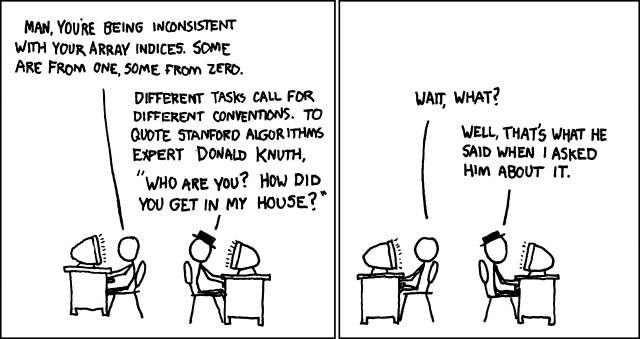
\includegraphics[width=4in]{donald_knuth.png}
    \caption*{His books were kinda intimidating; rappelling down through his skylight seemed like the best option.}
\end{figure}
\end{document}
